% !TeX program = lualatex
\lecture{3}{2025-02-24}{Fractional (Nointeger) Number}{}


\section{Fractional number}
\subsection{Fixed-Point Representation}
\begin{parag}{General Format}
    \begin{definition}
        Fixed-Point Numbers are:
        \begin{itemize}
            \item Integers
            \[I = -N, \dots, N\]
            \item Rational numbers ("\textit{binary}" rationals) of the form:
            \[x = \frac{a}{2^f}\]
            where $a \in I$ and $f$ positive integer
        \end{itemize}
    \end{definition}
    The fixed-point representation of a number $x$ consists of integer $x_{int}$ and fraction $x_{fr}$ components represented by $m$ and $f$ digits, respectively:
    \[x = x_{int} + x_{fr}\]
    \begin{definition}
        Digit-vector representation: 
        \[X = (X_{m-1}X_{m-2}\dots X_1X_0\underbrace{.}_{\text{Radix point}}X_{-1}X_{-2}\dots X_{-f})\]
        \begin{itemize}
            \item For \important{unsigned} numbers : 
            \[x = \sum_{i  = -f}^{m-1}X_i2^i\]
            \item For \important{signed} number in two's complement: 
            \[x = -X_{m-1}2^{m-1} + \sum_{i = -f}^{m-2}X_i2^i\]
        \end{itemize}
    \end{definition}
\end{parag}
\subsection{Radix point}
\begin{parag}{Separator between the integer and fractional parts}
    \[X = (X_{m-1}X_{m-2}\dots X_1X_0\underbrace{.}_{\text{Radix point}}X_{-1}X_{-2}\dots X_{-f})\]
    \begin{itemize}
        \item The position of the radix-point is assumed to be fixed
        \begin{itemize}
            \item Hence the name fixed-point
        \end{itemize}
        \item If the radix point is not shown, it is assumed to be to the right of the least significant digit (i.e, no fractional part)
        \begin{itemize}
            \item In that case, the number is an integer
        \end{itemize}
        \item Also known as decimal point, binary point, etc$\dots$
    \end{itemize}
\end{parag}
\begin{center}
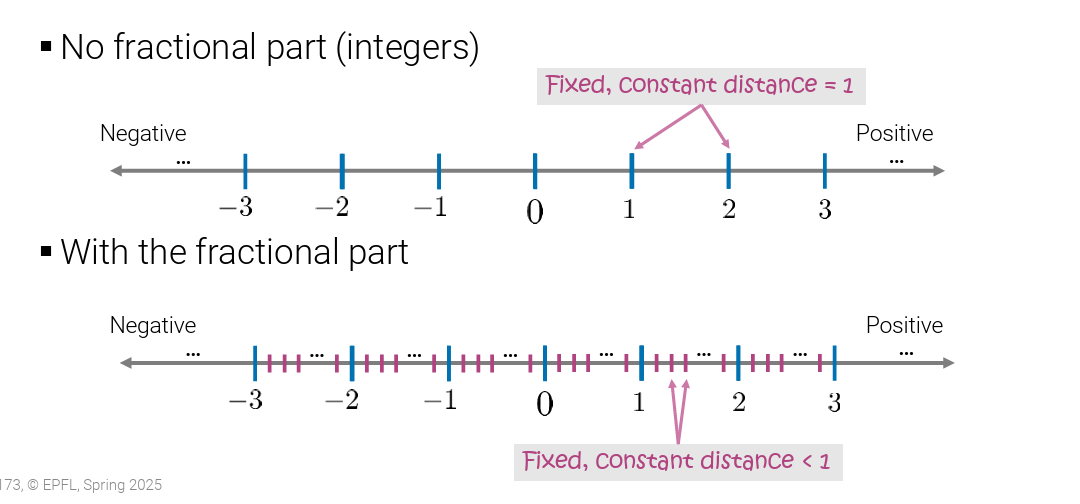
\includegraphics[scale=0.5]{Screenshot 2025-02-24 131346.png}
\end{center}

\
\begin{parag}{Example}
    \begin{itemize}
        \item Decimal number system and $m = 5, f = 5$
        \item Example decimal digit vector : 
            \begin{itemize}
                \item $X = (10077.01690)$
                \item $ x = 1 \cdot 10^4 + 7 \cdot 10^1 \cdots  + 0,009$
            \end{itemize}
        \item Most negative (min):
            \begin{align*}
                x_{min} = -99999.99999 = -99999 \frac{99999}{10^5}
            \end{align*}
            
        \item Largest number (max, positive):
            \begin{align*}
                x_{max} = +99999.99999 = +99999 \frac{99999}{10^5}
            \end{align*}

            
    \end{itemize}
    
\end{parag}



\begin{parag}{Fixed-point Representation}
    \begin{itemize}
        \item Given an unsigned fixed-point binary format $m = 3, f = 4$
            \begin{itemize}
                \item and an example binary digit vector:
                    \begin{align*}
                        X = (101.0111)
                    \end{align*}
                    
            \end{itemize}
        \item Q: Find the equivalent decimal number:
            \begin{align*}
                X = (101.0111); x = 2^2 + 2^0 + 2^{-2} + 2^{-3} + 2^{-4} = 5.4375
            \end{align*}
    \end{itemize}
    \begin{subparag}{Example}
        With sign-and-magnitude and $m = 5, f = 3$, Example of a binary digit vector:
        \begin{align*}
            X = (10101.110);\\
            x = -(4 + 1 + 0.5 + 0.25) = -5.75
        \end{align*}
        Therefore, The most negative number can be
        \begin{align*}
            x_{min} = 11111.111_2 = -15 \frac{7}{8}
        \end{align*}
        On the other hand, the largest number:
        \begin{align*}
            x_{max} = 01111.111 = 15 \frac{7}{8}
        \end{align*}
    \end{subparag}
    \begin{subparag}{Two's complement}
        With two's complement the work is the same as usual (the first digit is negative):
        \begin{align*}
            X =  (1010.1101); \\
            x = -8 + 2 + 0.5 + 0.0625 = -5.1875
        \end{align*}
        Here the most negative number is $x_{min} = 1000.0000_2 = -8$ and the largest one is $x_{max} = 0111.1111_2 = 7 \frac{15}{16}$
        
    \end{subparag}
\end{parag}
    \section{Concepts of finite precision math}
    \begin{parag}{Precision}
    \begin{definition}
        The precision is the maximum number of non-zero bits
    \end{definition}
    For example if we have $X = (X_{m-1}X_{m-2} \dots X_1 X_1 . X_{-1}X_{-2} \dots X_{-f}$ then, the precisions is the sum of $f$ and $m$:
    \begin{align*}
        \text{Precisions}(x) = m + f
    \end{align*}
    
    
    \end{parag}
   \begin{parag}{Resolution}
       \begin{definition}
           The resolution is the smallest possible difference between two consecutive numbers
       \end{definition}
       For example if a number as $f = 5$ (5 digits for is fractional part) then we know that the smallest possible difference between the number is $ \frac{1}{2^5} = \frac{1}{32}$ , for integer ($f = 0$) the resolution is $ \frac{1}{2^0} = 1$
   \\
   However, in the general case:
   \begin{align*}
       \text{Resolution(x)} = 2^{-f}
   \end{align*}

   
   \end{parag}
    
\begin{parag}{Rang}
    \begin{definition}
        The range is the difference between the most positive and the most negative number representable.
    \end{definition}
    For example with \important{two's complement}
    \\
    If we take, $m = 5, f = 3$, we compute $x_{max} = \sum_{i=-f}^{m-2}2^i = 15 \frac{7}{8}$, $x_{min} = -2^{m-1} = -16$. Then, the range is equal to $x_{max} - x_{min} = 31 \frac{7}{8}$
\\
In the general case, for fixed point and two's complement:
\begin{align*}
    \text{Range}(x) = x_{max} - x_{min} = \sum_{i-=f}^{m-2} 2^i - (-2^{m-1})
\end{align*}
\end{parag}
    \subsection{Accuracy}
    \begin{parag}{definition}
    \begin{definition}
        The accuracy is the magnitude of the maximum difference between a \textbf{real} value and its representation.
    \end{definition}
    
    The worst case (max difference) occurs for a real value exactly in the middle between two subsequent representable numbers (the real value lays between two equaly distant representation).
    \\
    In the general case = 
    \begin{align*}
        \text{Accuracy}(x) = \frac{ \text{Resolution} (x)}{2}
    \end{align*}    
    \end{parag}
    \begin{parag}{Dynamic Range}
        \begin{definition}
            The dynamic range is the \textbf{ratio} of, the maximum \textbf{absolute} value representable and the minimum positive value absolute (i.e nonzero) value representable.
        \end{definition}
        If we take the two's complement, with $m = 5, f=3$ then the maximum absolute value is $- -2^4 = 16$. For the minimum positive value we have $2^{-3} = \frac{1}{8}$. \\
    The dynamic range is said $ = \frac{x_{max}}{x_{min}} = 128$
In the general case, for fixed-point and two's complement:
\begin{align*}
    \text{Dynamic Range}(x) = \frac{2^{m-1}}{2^{-f}} = 2^{m-1 + f}
\end{align*}
\begin{subparag}{Personal remark}
    You can see as the \textit{size} of all the representable value divided by $2$, $128$. We have here $8$ bits which means that we have $2^8$ possible value which goes exactly to $256$.
\end{subparag}

        
    \end{parag}
    
\subsection{Floating-Point Number representation}
\begin{parag}{Floating-Point (FP) Representation}
    As with any other number representation in a digital system, $FP$ representation is encoded in a finite number of bits. It represents only a \important{finite subset} of the \important{infinite set} of real numbers.
    \\
    A real number that is \important{exactly} represented is called a \important{floating-point (FP) number}. All other real number either fall out of range (overflow or underflow) or are represented by $FP$ numbers that approximate their value. The process of approximation is called \important{roundoff} and produces a \important{roundoff error}.
    

\end{parag}

    \begin{parag}{Significand, Exponent, Base}
        $FP$ representation consists of two components : 
        \begin{itemize}
            \item the signed \important{significand} (also called \important{mantissa}) $M^*$
            \item the signed \important{exponent} $E$
                \begin{align*}
                    x = M^* \times b^E
                \end{align*}
                where $b$ is a constant called the \important{base}
                
        \end{itemize}
        Reminds us of the usual scientific notation, base $10$ :
        \begin{align*}
            +35200 = \underbrace{3.52}_{ \text{Coefficient}} \cdot 10^{+4} \; \; \; -0.099 = -9.9 \cdot \overbrace{10^{-2}}^{\text{Exponent}} 
        \end{align*}
        
    
    \end{parag}
    
    \begin{parag}{Benefits of Floating-Point}
        Consider $32$ bit two's complement signed integers:
        \begin{align*}
            \text{Dynamic Range}_1(x) = \frac{x_{max}}{x_{min}} = \frac{2^{32-1}}{2^0} = 2^31 \approx 2 \cdot 10^9
        \end{align*}
        New, let's consider alors a $32$ bit but floating-point number, with $24$-significand in sign and magnitude and $8$-bits exponent in two's complement.
        \begin{align*}
            \text{Dynamic Range}_2(x) = \frac{x_{max}}{x_{min}} = \frac{(2^{23}-1) \cdot 2^{2^{(8-1)}-1}}{2^0 \cdot2^{-2^{8-1}}} = (2^{23} - 1) \cdot2^{255} \approx 5 \cdot 10^{83}
        \end{align*}
        We can see here that the dynamic range increase a lot by a factor of $ \approx 10^{74}$
        
    
    \end{parag}
    
    \begin{parag}{Benefit}
        We can also see the benefits the resolution which also reduces of for example when taking a $32$-bits with $8$ fractional bits (fixed-point) and on the other side, $24$ bits significand in sign and magnitude and $8$ bit exponent in two's complement. If we compute each resolutions:
        \begin{align*}
            \text{Resolution}_1 (x) &= 2^{-8} = 0.00390625 \\
            \text{Resolution}_2(x) = 2^0 \cdot2^{-2^{(8-1)}} = 2^{-2^7} = 2^{-128}
        \end{align*}
        If we compute the ratio:
        \begin{align*}
            \frac{ \text{Resolution}_2(x)}{ \text{Resolution}_1(x)} = \frac{2^{-128}}{2^{-8}} = 2^{-120} \approx 7.523 \cdot 10^{-37}
        \end{align*}
        
    
    \end{parag}
   \subsection{Significand: Sign-and-Magnitude}
    
    \begin{parag}{Floating-Point Representation}
        Today, the most used representation for significand is sign and magnitude because it simplifies multiplication in hardware. 
        \\
        The floating-point representation becomes:
        \begin{align*}
            x = (-1)^S \times M \times b^E
        \end{align*}
        Where $S \in \{0, 1\}$ is the \important{sign} and $M$ is the \important{magnitude} of the signed significant
    \begin{framedremark}
        In the rest of the lecture, we assume significand is always represented in sign-and-magnitude.
    \end{framedremark}
    
    \end{parag}
    
    \begin{parag}{Digit vector}
        Many digit vectors are conceivable,  but we focus on the following:
        \begin{align*}
        X = ( \underbrace{SE_{m-1}}_{ \text{Sign}E_{m-2} \dots E_1 E_0 M_{n-1}M_{n-2} \dots M_0}
        \end{align*}
        Where $E_i$ is the exponent and $M_i$ is the magnitude.\\
        There is $(n+1)$ bit significand in \important{sign and magnitude} and $m$ bit exponent.
        
    
    \end{parag}
   \begin{parag}{Redundant}
       In the most general case, the representation: 
       \begin{align*}
           x = (-1)^S \times M \times b^E
       \end{align*}
       is redundant. Sign and magnitude is redundant, Multiple magnitude and exponent combinations can give the same number.
       \\
       \begin{subparag}{Example}
           If we take for example:
           \begin{align*}
               (1010)_2 \times 2^{-2} = 10 \times 2^{-2} = 2.5\\
               (0101)_2 \times 2^{-1} = 5 \times 2^{-1} = 2.5 \\
               (1.01)_2 \times 2^1 = 1.25 \times 2^1 = 2.5
           \end{align*}
           Floating-point representation is \important{redundant} \important{unless it is normalized}!
           \\
           If we take a magnitude that is \important{normalized}:
           \begin{align*}
               1 \leq M < 2
           \end{align*}
           Then: \begin{align*}
               1010.1000_2 = 1.0101_2 \times 2^3 = 10.5 \\
               -(0.00000011)_2 = -1.1_2 \times 2^{-7} = -0.01171875
           \end{align*}
          \begin{framedremark}
              Juste to be clearer, the normalized one here, is $1.0101_2 \times 2^3$ and $-1.1_2 \times 2^{-7}$. 
              \\
              For example let put $20_{10}$ normalized.
              \\
              First, $20_{10} = 10100_2$, however $ 1 \leq M < 2$, which leads us to: $1.0100_2 \times 2^4$. The $M$ being between $1$ and $2$ doesn't mean that the decimal number has a $1, \dots$.
          \end{framedremark}
       \end{subparag}
       
   
   \end{parag}
    
   \begin{parag}{Hidden Bit and Fraction}
       As the significand is normalized, the first digit of the magnitude is \important{always} binary $1$. If something is always the same, it can be omitted (saving precious bits)\\
       The first digit of the significand is omitted and called \important{hidden bit}. \\
       The binary point is assumed to the right of the hidden bit. The represented part of the significand is called \important{fraction F}.
   
       \begin{subparag}{Example}
           \begin{align*}
               \overbrace{101.001_2}^{ \text{unormalized significand}} \times 2^{-4}  = \underbrace{1.01001_2}_{ \text{Normalized significand}} \times 2^{-2} = \overbrace{.01001_2}^{ \text{hidden is not represented}} \times 2^{-2}
           \end{align*}
           
           
       \end{subparag}
   \end{parag}
   \begin{parag}{Summary}
       \begin{itemize}
           \item Common significand representation is the following:
               \begin{itemize}
                   \item Sign-and-magnitude
                   \item Normalized
                   \item One hidden bit
               \end{itemize}
           \item Corresponding significand value becomes:
               \begin{align*}
                   (-1)^S \times (1 + \sum_{i=1}^n M_{n-1} 2^{-1})
               \end{align*}
               
       \end{itemize}
   
   \end{parag}
   
      \section{Exponent}
      \begin{parag}{Exponent}
          Exponent needs to be signed
          \begin{itemize}
              \item \important{Positive} for representing very large numbers ( \important{large absolute} value)
              \item \important{Negative} for representing very small numbers ( \important{small absolute} value)
          \end{itemize}
      
      \end{parag}
      
      \begin{parag}{Biased representation}
          Exponent can take any signed representation we know but there is one particular representation, called \important{biased}, which simplifies comparing two $FP$ numbers in hardware.
          \\
          Biased representation of a digit vector $X = (X_{n-1} \dots X_1 X_0)$
          \begin{align*}
              x = \sum_{i=0}^{n-1} X_i 2^i - B
          \end{align*}
          
          Typically, the bias equals $B = 2^{n-1} - 1$
      
      \end{parag}
     \begin{parag}{Biased representation, Cntd.}
         Where's the catch?
         \begin{itemize}
             \item Resulting number are sorted just like unsigned integers but cover both the positive and negative numbers
             \item efficient hardware (superior to two's complement)
             \item Min exponent is represented as all zeros
             \begin{itemize}
                 \item $FP$ zero can be represented as all zeros (significand and exponent)
             \end{itemize}
         \end{itemize}

     
     \end{parag}
      
\subsubsection{Summary}
\begin{parag}{Exponent}
    \begin{itemize}
        \item Common representation of an -$m$ bit exponent is biased with base $B = 2^{m-1}-1$
        \item For the binary digit vector:
            \begin{align*}
                X = (SE_{m-1}E_{m-2} \dots E_1E_0 . M_{n-1}M_{n-2} \dots M_0)
            \end{align*}
            this biased exponent \textbf{value} becomes : 
            \begin{align*}
                e = \sum_{j=0}^{m-1} E_j 2^j - (2^{m-1} - 1)
            \end{align*}
            
    \end{itemize}

\end{parag}
\begin{parag}{Floating point format}
    There could be many floating point formats, but we will often assume:
   \begin{itemize}
       \item $(n+1)$-bit significand 
       \item Sign and magnitude
       \item Normalized, one hidden bit
   \end{itemize}
   \begin{itemize}
       \item $m$-bit exponent
           \begin{itemize}
               \item Biased, $B = 2^{m-1} -1$
           \end{itemize}
   \end{itemize}
   \begin{align*}
       X = (SE_{m-1}E_{m-2} \dots E_1 E_0 . M_{n-1} M_{n-2} \dots M_0)
   \end{align*}
   \begin{align*}
       x = (-1)^S \times (1 + \sum_{i=1}^n M_{n-i}2^{-i}) \times 2^{\sum_{j=0}^{m-1} E_j 2^j - (2^{m-1}-1)}
   \end{align*}
   
   

\end{parag}

    \section{Rounding}
    The result of a floating-point operation is a real number that, to be represented exactly might require a significand with an infinite number of digits.\\
    To obtain a representation close to the exact result, we perform what is called \important{rounding}
    \begin{parag}{Rounding modes}
        Various rounding modes exist
        \begin{itemize}
            \item Round to \important{nearest}, to \important{even} when \important{tie}
            \item Round towards \important{zero} (truncate)
            \item Round towards plus or towards minus \important{infinity}
        \end{itemize}
        Consider the real number $x_{real}$ and the consecutive floating-point number $F_1$ and $F_2$ \text{ such that }$F_1 \leq x_{real} \leq F_2$, we round it like always (normal definition)
      
    \end{parag}
    
    
    \subsection{IEE Standard 754}
        \begin{parag}{$FP$ format in IEEE 754}
            Exactly what we described
            \begin{itemize}
                \item $(n+1)-$bit significand
                    \item Sign and magnitude, Normalized, one hidden bit
                    \item $m$-bit exponent 
                        \begin{itemize}
                            \item Biased $B = 2^{m-1} - 1$
                        \end{itemize}
            \end{itemize}
            \begin{align*}
                X = (SE_{m-1}E_{m-2} \dots E_1E_0 . M_{n-1}M_{n-2} \dots M_0)
            \end{align*}
    There is two types of formats: Basic and extended format:
    \begin{subparag}{Basic formats}
        \begin{itemize}
            \item Sign $S$ $1$ bit
            \item Exponent $E$: $8$ bits
            \item Fraction $F$: $23$ bits
        \end{itemize}
        The default rounding mode is to the nearest, to even when there is a tie.
    \end{subparag}
    \begin{subparag}{Double precision (64 bits)}
        \begin{itemize}
            \item Sign $S$: 1 bit
            \item Exponent $E$: $11$ bits
            \item Fraction $F$: 52 bits
        \end{itemize}
        
        
    \end{subparag}
        \end{parag}
        
        \begin{parag}{Special Values}
            \begin{itemize}
                \item Floating-point \important{zero}: $E = 0, F = 0$
                    \begin{itemize}
                        \item The sign $S$ differentiates between positive and negative zero, Value $1.0 \times 2^{-B}$ is not represented.
                    \end{itemize}
                \item Positive and negative \important{infinity}
                    \begin{itemize}
                        \item Biased exponents all ones, $F = 0$
                       
                    \end{itemize}
                \item \important{NaN} (not a number)
                    \begin{itemize}
                        \item To represent results of invalid operations(for example, the square root of a negative number)
                        \item Sign $= 0$ or $1$ biased exponents all ones, $F \neq 0$
                    \end{itemize}
            \end{itemize}
        \end{parag}
        
        \begin{parag}{Exceptions: Handling of special situations}
            The following five exceptions set a flag (i.e " \textit{activate an alarm}") and the computation continues.
            \begin{itemize}
                \item \important{Overflow}, when the rounded value is \textbf{to large} to be represented 
                    \begin{itemize}
                        \item Result is set to infinity
                    \end{itemize}
                \item \important{Underflow}, when the rounded value is to small to be represented
            s to small to be represented
        \item Division by zero
        \item Inexact result, when the result is not an exact floating-point number
        \item invalid result, When $NaN$ is produce by zero
                \item Inexact result, when the result is not an exact floating-point number
                \item invalid result, When $NaN$ is produced
            \end{itemize}
        
        \end{parag}
        
